\documentclass[a4paper]{article}
\usepackage[14pt]{extsizes} 
\usepackage[T2A]{fontenc}
\usepackage[utf8]{inputenc}
\usepackage{natbib}
\usepackage{graphicx}
\usepackage{amsmath}
\usepackage[english]{babel}
\usepackage{fontspec}
\usepackage{amsmath,amsfonts,amssymb,amsthm,mathtools,mathrsfs}
\usepackage{icomma}
\usepackage{fullpage}
\usepackage{ulem}
\usepackage{eufrak}
\usepackage{setspace}
\usepackage{listings}
\usepackage{indentfirst}
\usepackage[left=2cm,right=1.5cm,top=2cm,bottom=2cm]{geometry}
\usepackage{xcolor}
\usepackage{float}
\usepackage{csquotes}

\setmainfont[Ligatures={TeX,Historic}]{Times New Roman}
\setlength{\parindent}{5ex}
\setlength{\parskip}{1em}
\renewcommand{\baselinestretch}{1}

\graphicspath{{images/}}

\definecolor{buzzlightyear}{HTML}{8757A5}
\definecolor{grass}{HTML}{738D06}
\definecolor{literal}{HTML}{F18A2B}
\definecolor{commentcolor}{HTML}{8E908B}

\lstdefinestyle{habrstyle}{
    backgroundcolor=\color{white},   
    commentstyle=\color{commentcolor},
    keywordstyle=\bfseries\color{buzzlightyear},
    numberstyle=\tiny\color{commentcolor},
    stringstyle=\color{grass},
    basicstyle=\ttfamily\footnotesize,
    breakatwhitespace=false,         
    breaklines=true,                 
    captionpos=b,                    
    keepspaces=true,                 
    numbers=left,                    
    numbersep=5pt,                  
    showspaces=false,                
    showstringspaces=false,
    showtabs=false,                  
    tabsize=4
}

\lstset{style=habrstyle}

\begin{document}

    % FIRST PAGE
    \begin{center}
        \begin{center}
        \hfill \break
        \normalsize{Санкт-Петербургский государственный политехнический}\\
        \normalsize{университет Петра Великого}\\
        \hfill \break
        \normalsize{\textbf{Высшая школа интеллектуальных систем и}}\\ 
        \normalsize{\textbf{суперкомпьютерных технологий}}\\ 
        \hfill \break
        \hfill \break
        \hfill \break
        \normalsize{Лабораторная работа}\\
        \hfill \break
        \hfill \break
        \normalsize{\LARGE Фильтрация и свертка}\\
        \end{center}
        \hfill \break
        \hfill \break
        \hfill \break
        \hfill \break
        \hfill \break
        \hfill \break
        \hfill \break
        \hfill \break
        \hfill \break
        \hfill \break
        \begin{flushright}
            \normalsize{Работу выполнил студент}\\
            \normalsize{3-го курса, группа 3530901/80201}\\
            \normalsize{Сахибгареев Рамис Ринатович}\\
            \hfill \break
            \normalsize{Преподаватель:}\\
            \normalsize{Богач Наталья Владимировна}\\
        \end{flushright}
        \hfill \break
        \hfill \break
        \hfill \break
        \hfill \break
        \begin{center} Санкт-Петербург 2021 \end{center}
        \thispagestyle{empty}
    \end{center}
    % FIRST PAGE [END]
    
    \newpage
        \tableofcontents
    
    \newpage
         \listoffigures
    
    \newpage
         \lstlistoflistings   
     
    % START START START START START
    \newpage
        \section{Part 1: Research and execution of chap08}
        
        In this part we need to research and execute existing chap08.ipynb file, that contains information windows and auto-correlation.
        
        File was successfully executed. Window - is a wa to smooth signal, make it less "noisy". Convolution window can be showed as amplitude to frequency ratio.
        
        \begin{figure}[H]
            \centering
            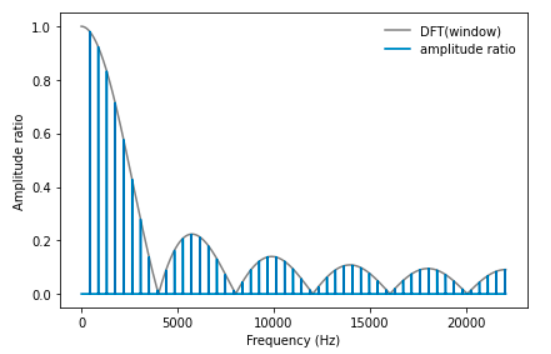
\includegraphics[width=\textwidth]{img/p1_1.png}
            \caption{Ampltude to frequency ratio}
            \label{fig:p1_2}
        \end{figure}
        
        We can test Gaussian Window by increasing standard deviation. We can see, as we increasing the standard deviation, "боковые лепестки" increasing too. It happens, because Gaussian Window becomes more and more flat.
        
        \begin{figure}[H]
            \centering
            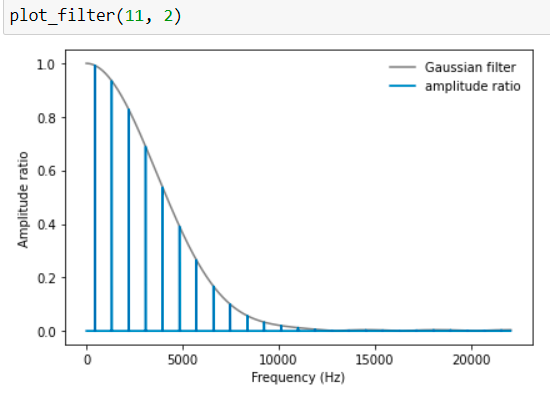
\includegraphics[width=\textwidth]{img/p1_2.png}
            \caption{Gaussian window result (std = 2)}
            \label{fig:p1_1}
        \end{figure}
        
        \begin{figure}[H]
            \centering
            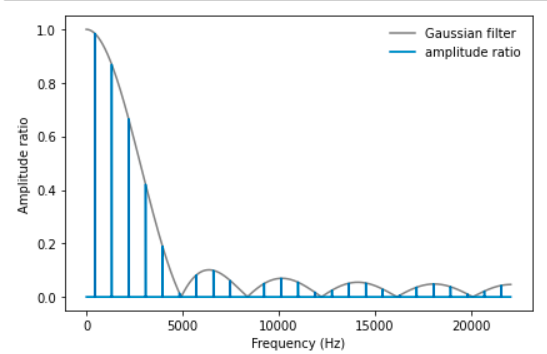
\includegraphics[width=\textwidth]{img/p1_3.png}
            \caption{Gaussian window result (std = 4}
            \label{fig:p1_1}
        \end{figure}
        
        \begin{figure}[H]
            \centering
            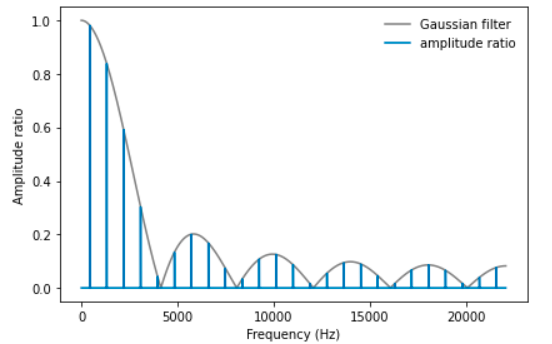
\includegraphics[width=\textwidth]{img/p1_4.png}
            \caption{Gaussian window result (std = 10}
            \label{fig:p1_1}
        \end{figure}
        
    \newpage
        \section{Part 2: FFT on Gaussian}

        In this part we need to perform FFT on Gaussian curve with different standard deviation. Take into account, that plotting function rolls the FFT result, so we can clearly see gaussian. Actual zero frequency = half of plot frequency.
        
        \begin{lstlisting}[language=Python,caption=Plotting function,label={lst:part1_2}]
    def plot_gaussian(std):
        M = 64
        gaussian = scipy.signal.gaussian(M=M, std=std)
        gaussian /= sum(gaussian)
        
        plt.subplot(1, 2, 1)
        plt.plot(gaussian)
        decorate(xlabel='Time')
    
        fft_gaussian = np.fft.fft(gaussian)
        fft_rolled = np.roll(fft_gaussian, M//2)
        
        plt.subplot(1, 2, 2)
        plt.plot(np.abs(fft_rolled))
        decorate(xlabel='Frequency')
        plt.show()
        \end{lstlisting}
        
        \begin{figure}[H]
            \centering
            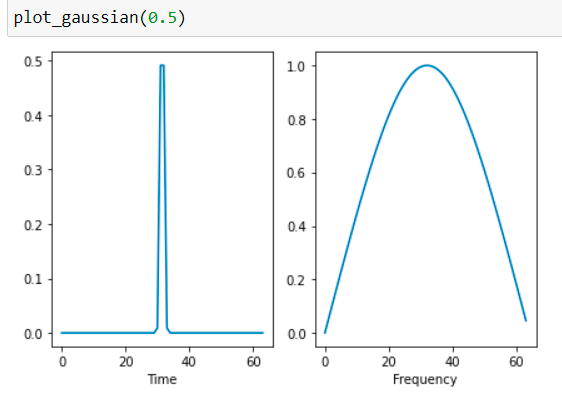
\includegraphics[width=\textwidth]{img/p2_1.png}
            \caption{std = 0.5}
            \label{fig:part1_1_2}
        \end{figure}
        
        \begin{figure}[H]
            \centering
            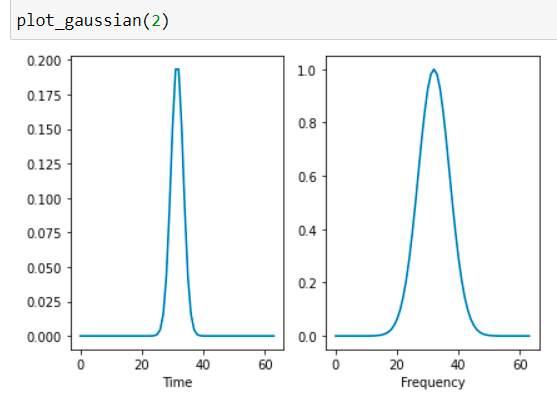
\includegraphics[width=\textwidth]{img/p2_2.png}
            \caption{std = 2}
            \label{fig:part1_1_2}
        \end{figure}
        
        \begin{figure}[H]
            \centering
            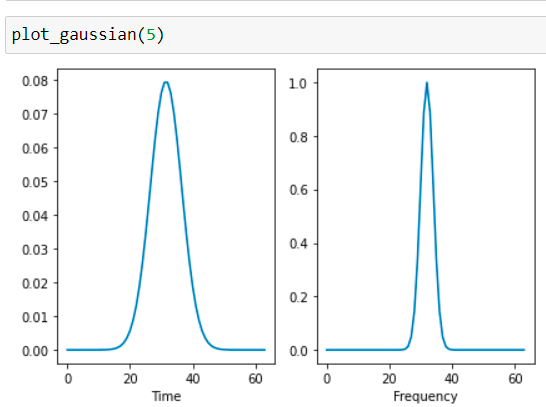
\includegraphics[width=\textwidth]{img/p2_3.png}
            \caption{std = 5}
            \label{fig:part1_1_2}
        \end{figure}
        
        \begin{figure}[H]
            \centering
            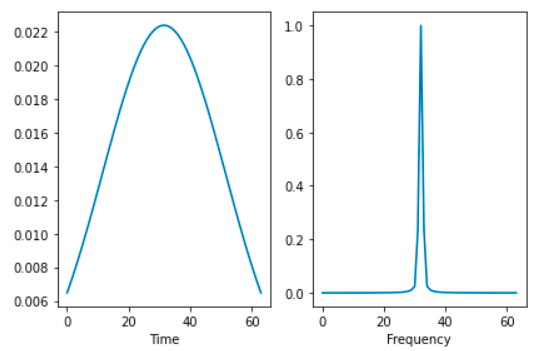
\includegraphics[width=\textwidth]{img/p2_4.png}
            \caption{std = 20}
            \label{fig:part1_1_2}
        \end{figure}
        
        We can clearly see, that by increasing standard deviation Gaussian curve becomes more flat and more looks like part of sin function. That's why frequency becomes more "clear" and concentrates around zero.
            
    \newpage
        \section{Different windows comparison}
        
            In this part, we need to compare different windows as they are good as a low-pass filter. Blackman, Gaussian, Hanning, Hamming, Bartlett filters was used.
            
            \begin{lstlisting}[language=Python,caption=Plotting code,label={lst:part1_2}]
    signal = SquareSignal(freq=440)
    wave = signal.make_wave(duration=1.0, framerate=441000)
    
    M = 30
    gaussian = scipy.signal.gaussian(M=M, std=2.5)   
    bartlett = np.bartlett(M)
    blackman = np.blackman(M)
    hamming = np.hamming(M)
    hanning = np.hanning(M)
    
    windows = [blackman, gaussian, hanning, hamming, bartlett]
    names = ['blackman', 'gaussian', 'hanning', 'hamming', 'bartlett']
    for window in windows:
        window /= sum(window)
        
    for window, name in zip(windows, names):
        plt.plot(window, label=name)
        decorate(xlabel='Index')
    
    for window, name in zip(windows, names):
        padded =  zero_pad(window, len(wave))
        plt.plot(abs(np.fft.rfft(padded)), label=name)
        decorate(xlabel='Frequency')
        plt.ylim(top=0.1)
        plt.xlim(right = 20000)
        \end{lstlisting}
        
        \begin{figure}[H]
            \centering
            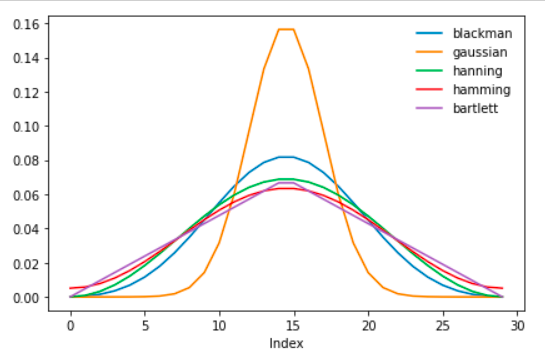
\includegraphics[width=\textwidth]{img/p3_1.png}
            \caption{Resulting windows}
            \label{fig:part1_1_2}
        \end{figure}
        
        \begin{figure}[H]
            \centering
            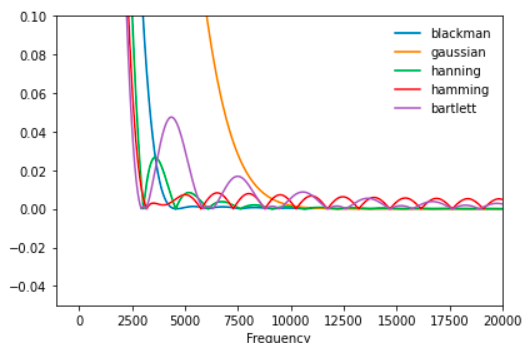
\includegraphics[width=\textwidth]{img/p3_2.png}
            \caption{Resulting DFT plots}
            \label{fig:part1_1_2}
        \end{figure}
        
        \begin{figure}[H]
            \centering
            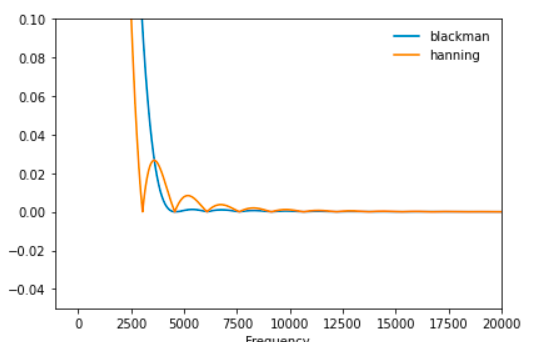
\includegraphics[width=\textwidth]{img/p3_3.png}
            \caption{Hanning and Blackman side by side}
            \label{fig:part1_1_2}
        \end{figure}
        
        We can see, that a Gaussian window drops off slow, but it most consistent and "smooth". However, there are good alternatives: a Hanning and a Blackman windows. They both drop off faster, than a Gaussian window, but also pretty smooth. Blackman window drops a bit slower, than a Hanning one, but it has much less "bumps".
            
    \newpage
        \section{Conclusion}
            We've learned, what is filtering windows and autocorrelation. We've made some test, to find out how different standard deviation affects the Gaussian window: with big standard deviation values Gaussian filter is very "bumpy" and "unsmooth". We've discovered, that DFT of a Gaussian curve is a Gaussian curve also, but with reversed standard deviation. We've compared different windows as they are good as a low-pass filter. The result is that answer is complex: it can be a Blackman window, if we need to have a very smooth filter with pretty fast drop off, or it can be a Hanning window if we need very fast drop off, but we can have some unsmootheness in out filter.
     
\end{document}
